\documentclass[tikz, border=5mm]{standalone}
\usepackage{amsmath}
\usetikzlibrary{calc, decorations.pathreplacing}

\begin{document}
	
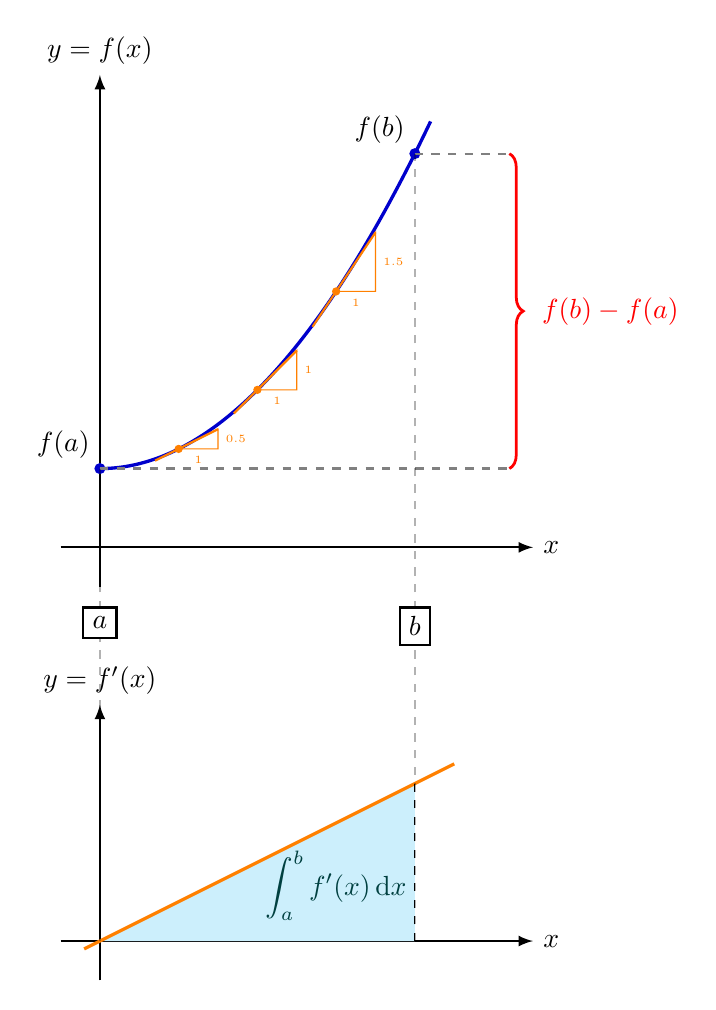
\begin{tikzpicture}[>=latex, font=\sffamily, thick]
	
	% --- Constants ---
	\def\xa{0}
	\def\xb{4}
	\def\ysep{5.0}
	
	% Pre-calculate Key Y-values
	\pgfmathsetmacro{\ya}{0.25*\xa*\xa + 1}
	\pgfmathsetmacro{\yb}{0.25*\xb*\xb + 1}
	\pgfmathsetmacro{\yprimeb}{0.5*\xb}
	
	% =======================================================
	% TOP GRAPH: f(x) with SLOPE TRIANGLES
	% =======================================================
	\begin{scope}[yshift=\ysep cm]
		% Axes
		\draw[->] (-0.5, 0) -- (5.5, 0) node[right] {$x$};
		\draw[->] (0, -0.5) -- (0, 6) node[above] {$y = f(x)$};
		
		% Function Curve
		\draw[blue!80!black, line width=1.2pt] 
		plot[domain=0:4.2, samples=100] (\x, {0.25*\x*\x + 1});
		
		% --- DETAILED SLOPE TRIANGLES LOOP ---
		\foreach \i in {1, 2, 3} {
			\pgfmathsetmacro{\ix}{\i}
			\pgfmathsetmacro{\iy}{0.25*\ix*\ix + 1}
			\pgfmathsetmacro{\slope}{0.5*\ix}   % m = 0.5, 1.0, 1.5
			\pgfmathsetmacro{\run}{0.5}         % Horizontal step size
			\pgfmathsetmacro{\rise}{\slope*\run} % Vertical step size
			
			% 1. Draw the Triangle (Teal lines)
			% Path: Start -> Right -> Up -> Back to Start
			\draw[orange, thin] 
			(\ix, \iy) 
			-- (\ix + \run, \iy) node[midway, below, font=\tiny, scale=0.8] {1} 
			-- (\ix + \run, \iy + \rise) node[midway, right, font=\tiny, scale=0.8] {$\pgfmathprintnumber{\slope}$}
			-- cycle;
			
			% 2. Extend the tangent line backwards for better look
			\draw[orange, thick] (\ix, \iy) -- (\ix - 0.3, \iy - \slope*0.3);
			% 3. Re-draw the hypotenuse thick to match
			\draw[orange, thick] (\ix, \iy) -- (\ix + \run, \iy + \rise);
			
			% 4. Dot
			\fill[orange] (\ix, \iy) circle (1.5pt);
		}
		
		% Points and Brace
		\fill[blue!80!black] (\xa, \ya) circle (2pt);
		\fill[blue!80!black] (\xb, \yb) circle (2pt);
		
		\draw[dashed, gray] (\xa, \ya) -- (5.2, \ya);
		\draw[dashed, gray] (\xb, \yb) -- (5.2, \yb);
		
		\draw[decorate, decoration={brace, amplitude=5pt, mirror}, red, line width=1pt]
		(5.2, \ya) -- (5.2, \yb)
		node[midway, right=8pt, align=left] {$f(b) - f(a)$};
		
		\node[above left] at (\xa, \ya) {$f(a)$};
		\node[above left] at (\xb, \yb) {$f(b)$};
	\end{scope}
	
	% =======================================================
	% BOTTOM GRAPH: f'(x)
	% =======================================================
	\begin{scope}
		\draw[->] (-0.5, 0) -- (5.5, 0) node[right] {$x$};
		\draw[->] (0, -0.5) -- (0, 3) node[above] {$y = f'(x)$};
		
		\fill[cyan!20] (\xa, 0) -- plot[domain=\xa:\xb] (\x, {0.5*\x}) -- (\xb, 0) -- cycle;
		\draw[orange, line width=1.2pt] (-0.2, -0.1) -- (4.5, 2.25);
		\node[teal!50!black] at (3, 0.7) {$\displaystyle \int_a^b f'(x)\,\mathrm{d}x$};
		\draw[dashed, thin] (\xb, 0) -- (\xb, \yprimeb);
	\end{scope}
	
	% =======================================================
	% CONNECTING LINES
	% =======================================================
	\draw[dashed, opacity=0.3] (\xa, 0) -- (\xa, \ya+\ysep);
	\draw[dashed, opacity=0.3] (\xb, 0) -- (\xb, \yb+\ysep);
	
	\node[below, draw=black, fill=white] at (\xa, 4.25) {$a$};
	\node[below, draw=black, fill=white] at (\xb, 4.25) {$b$};
	
\end{tikzpicture}
	
\end{document}